\chapter{Tổng kết: bức tranh toàn cảnh}
\label{ch:tongket}

\section{Một biểu đồ cho tất cả}

Hình~\ref{fig:tongket} đặt mọi phương pháp đã chạy trong tài liệu lên cùng một thước đo: sai số năng lượng của nguyên tử Li so với đáp án 15 chữ số. Trục hoành dùng thang log, mỗi vạch chia là một bậc độ chính xác (gấp 10 lần).

\begin{figure}[h]
\centering
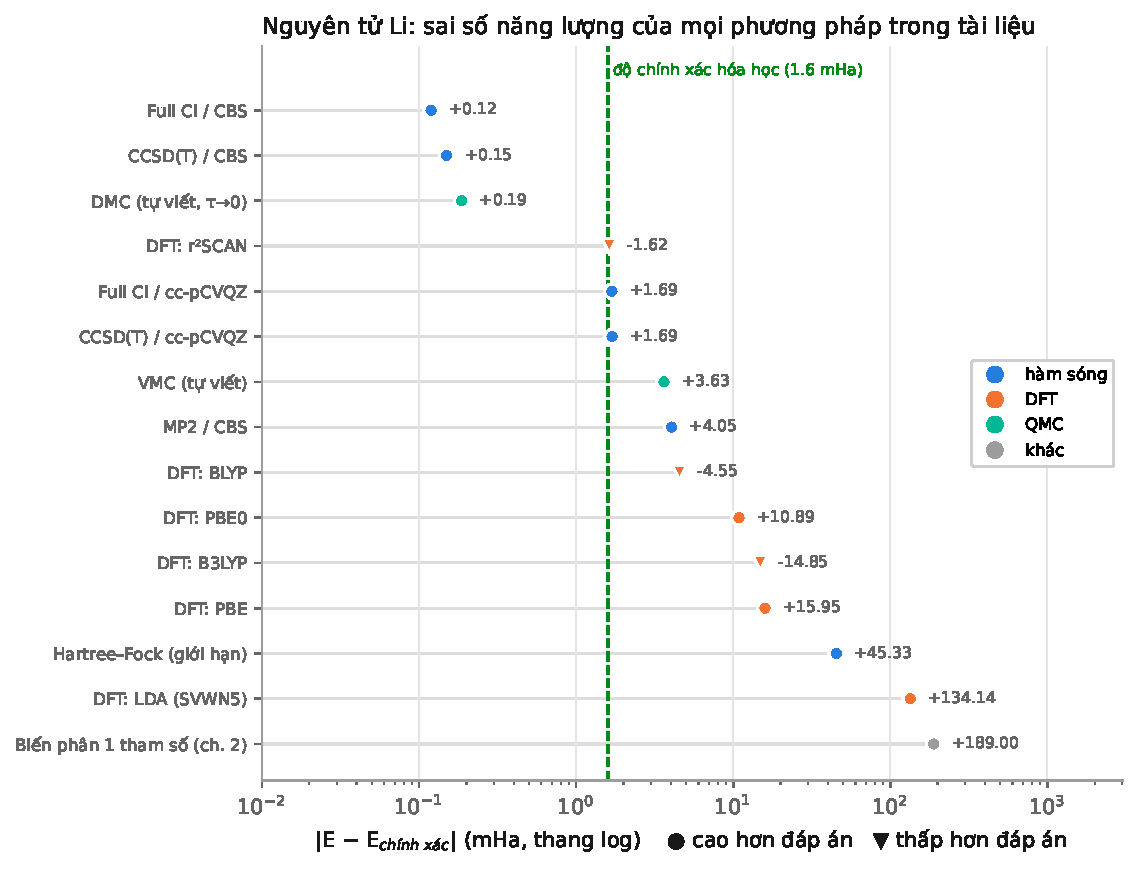
\includegraphics[width=\textwidth]{06_tong_ket.pdf}
\caption{Sai số năng lượng của Li với mọi phương pháp trong tài liệu, sắp xếp từ chính xác nhất (dưới) tới kém nhất (trên). Màu theo họ phương pháp: xanh dương là hàm sóng, cam là DFT, xanh ngọc là Monte Carlo lượng tử tự viết. Hình tròn: cao hơn đáp án; tam giác: thấp hơn đáp án (chỉ xảy ra với DFT và với sai số thống kê của DMC). Vạch xanh lá: độ chính xác hóa học. (Script \code{06\_tong\_hop.py})}
\label{fig:tongket}
\end{figure}

\section{Bảng so sánh}

\begin{table}[h]
\centering\small
\caption{So sánh các phương pháp. Cột ``Li'' là sai số năng lượng toàn phần tính bằng code đi kèm (mHa).}
\label{tab:tongket}
\begin{tabularx}{\textwidth}{@{}l>{\raggedright\arraybackslash}X>{\raggedright\arraybackslash}p{1.6cm}r>{\raggedright\arraybackslash}X@{}}
\toprule
Phương pháp & Xấp xỉ điều gì & Chi phí & Li & Dùng khi nào \\
\midrule
Hartree--Fock & Một định thức; electron khác spin không né nhau & $N^4$ & $+45.3$ & Điểm xuất phát cho mọi phương pháp hàm sóng \\
MP2 & Tương quan như nhiễu loạn bậc 2 & $N^5$ & $\ErrMPtwoCBS$ & Ước lượng nhanh tương quan (CBS) \\
CCSD(T) & Kích thích đơn, đôi (lặp) + ba (nhiễu loạn) & $N^7$ & $\ErrCCSDTCBS$ & Chuẩn vàng cho phân tử nhỏ, vừa, đơn tham chiếu (CBS) \\
Full CI & Không xấp xỉ, chỉ giới hạn bởi tập cơ sở & $e^N$ & $\ErrFciCBS$ & Hệ rất nhỏ; làm chuẩn để kiểm tra (CBS) \\
LDA & Mỗi điểm như khí electron đồng nhất & $N^3$ & $\ErrLDA$ & Chủ yếu cho chất rắn, lịch sử \\
PBE & Thêm độ dốc mật độ & $N^3$ & $\ErrPBE$ & Vật liệu, chất rắn, hệ lớn \\
B3LYP & Thêm 20\% trao đổi chính xác & $N^4$ & $\ErrBthreeLYP$ & Hóa học phân tử thường ngày \\
VMC & Dạng hàm thử (Slater--Jastrow) & $N^3$--$N^4$ & $\ErrVmc$ & Kiểm tra, tối ưu hàm thử \\
DMC & Nút của hàm thử & $N^3$--$N^4$ & $\ErrDmc$ & Độ chính xác cao, hệ lớn, song song tốt \\
Mạng nơ-ron & Kiến trúc và quá trình huấn luyện & $N^4$ & --- & Nghiên cứu: hệ nhỏ, vừa, cực chính xác \\
Máy lượng tử & Số qubit, nhiễu, độ sâu mạch & --- & --- & Nghiên cứu; tương lai cho tương quan mạnh \\
\bottomrule
\end{tabularx}
\end{table}

\section{Bốn chiến lược vượt bức tường hàm mũ}

Nhìn lại toàn bộ tài liệu, mọi phương pháp đều là một cách ``lách'' bức tường hàm mũ của chương~\ref{ch:baitoan}. Có bốn chiến lược chính:

\begin{enumerate}
\item \textbf{Thu hẹp dạng hàm sóng.} Không cho hàm sóng tự do, mà chỉ tìm trong một ``lớp'' hàm có cấu trúc: một định thức (HF), định thức nhân $e^{\hat T}$ cắt ngắn (CC), định thức nhân thừa số Jastrow (VMC). Số tham số chỉ tăng theo đa thức. Cái giá: sai số do chọn lớp hàm.
\item \textbf{Đổi biến.} Thay hàm sóng $3N$ chiều bằng mật độ 3 chiều (DFT). Bài toán trở nên rẻ, nhưng mọi khó khăn dồn vào phiếm hàm $E_{xc}$ chưa biết.
\item \textbf{Lấy mẫu ngẫu nhiên.} Không lưu hàm sóng, chỉ lấy mẫu nó (QMC). Sai số thống kê giảm như $1/\sqrt M$ bất kể số chiều. Cái giá: bài toán dấu của fermion, xử lý gần đúng bằng nút cố định.
\item \textbf{Biểu diễn mới.} Dùng các cấu trúc dữ liệu có khả năng nén thông tin tốt hơn: mạng nơ-ron, mạng tensor, hay trạng thái của chính một hệ lượng tử khác (máy tính lượng tử). Chương~\ref{ch:biengioi} trình bày các hướng này.
\end{enumerate}

\begin{eli5}[bốn cách xếp hành lý]
Bạn phải mang theo một ``tủ quần áo'' khổng lồ (hàm sóng chính xác) mà không vali nào chứa nổi. Cách 1: chỉ mang những bộ đồ theo vài kiểu cố định (thu hẹp dạng hàm). Cách 2: chỉ mang tấm ảnh chụp tủ quần áo, rồi dùng ``công thức'' để suy ra mọi thứ khác (đổi biến, DFT). Cách 3: mỗi ngày bốc ngẫu nhiên vài bộ, đủ để biết ``trung bình'' bạn mặc gì (lấy mẫu). Cách 4: phát minh ra một loại vali hút chân không nén được quần áo (biểu diễn mới).
\end{eli5}

\section{Điều gì đã giải quyết, điều gì còn mở?}

\paragraph{Đã giải quyết khá tốt.}
Nguyên tử và phân tử nhỏ mà hàm sóng có một cấu hình chiếm ưu thế, như Li trong tài liệu này: CCSD(T) ngoại suy về tập cơ sở vô hạn và DMC đều đạt độ chính xác hóa học. Với hệ lớn hơn (hàng trăm, hàng nghìn nguyên tử), DFT cho kết quả ``đủ dùng'' với chi phí chấp nhận được.

\paragraph{Còn mở.}
\begin{itemize}
\item \textbf{Tương quan mạnh}: khi nhiều cấu hình quan trọng ngang nhau (kim loại chuyển tiếp, liên kết bị kéo giãn, chất siêu dẫn nhiệt độ cao, vật liệu từ), cả CCSD(T) lẫn DFT thông thường đều thất bại, còn các phương pháp đa tham chiếu lại tăng chi phí theo hàm mũ.
\item \textbf{Hệ lớn với độ chính xác cao}: đưa độ chính xác cỡ CCSD(T) hay DMC tới protein, bề mặt xúc tác, vật liệu thực.
\item \textbf{Một phiếm hàm DFT ``tốt cho mọi thứ''}: chưa có, và không có con đường cải thiện có hệ thống.
\item \textbf{Bài toán dấu}: chưa có cách giải tổng quát, và có lý do lý thuyết (NP-khó) để tin rằng sẽ không có \cite{TroyerWiese2005}.
\end{itemize}

\section{Lời kết}

Ta bắt đầu từ câu nói của Dirac năm 1929: các định luật đã biết hết, chỉ có phương trình là quá phức tạp để giải. Gần một thế kỷ sau, điều đó vẫn đúng, nhưng ta đã đi được một chặng rất dài. Với nguyên tử Li, một chương trình Hartree--Fock 30 dòng cho 99.4\% năng lượng. Full CI trên máy tính xách tay cùng phép ngoại suy thông minh đạt sai số $\ErrFciCBS\mHa$. Một chương trình Monte Carlo vài trăm dòng tự viết đạt độ chính xác tương đương mà không cần tập cơ sở nào. Mỗi phương pháp là một ý tưởng vật lý đẹp: trường trung bình, phản đối xứng, lãi kép, mật độ thay cho hàm sóng, mực loang trong thời gian ảo.

Nếu bạn muốn đi tiếp, Phụ lục~\ref{pl:lotrinh} có lộ trình chi tiết, Phụ lục~\ref{pl:tailieu} có tài liệu nên đọc, và thư mục \code{code/} là nơi tốt nhất để bắt đầu: sửa một tham số, chạy lại, và xem điều gì thay đổi.
